\begin{frame}
  \frametitle{Dirichlet distribution}
  \begin{center}
    Rolling a die is a probability distribution over the numbers from 1 to 6.

    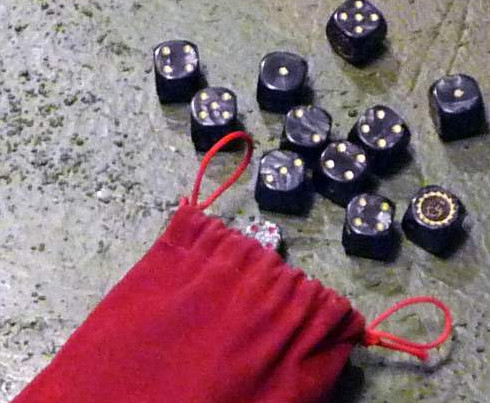
\includegraphics[width=0.6\textwidth]{img/dice2-cropped.jpg}

    Selecting a die from a bag of dice is a probability distribution over the dice.

    The Dirichlet distribution models this.
  \end{center}
\end{frame}

\begin{frame}
  \frametitle{Normal distribution}
  \begin{center}
    The normal distribution is good for things like environmental noise models.

    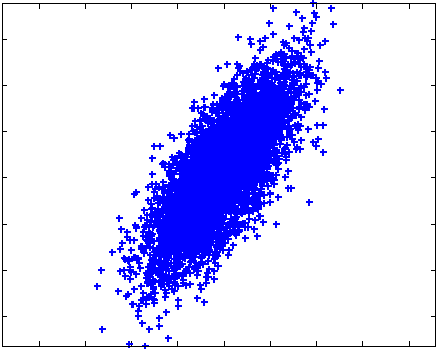
\includegraphics[width=0.6\textwidth]{img/normal.png}

    Unlike the Dirichlet distribution, it can model correlations between different variables.
  \end{center}
\end{frame}

\begin{frame}
  \frametitle{Logistic transformation}
  \begin{columns}
    \begin{column}{0.65\textwidth}
      \begin{center}
        \begin{itemize}
          \item The Dirichlet distribution is a probability distribution over probability distributions
                (like the bag of dice), but doesn't model correlations.

          \item The normal distribution models correlations, but is a distribution over vectors in $\mathbb{R}_n$.

          \item The logistic transformation can be applied to the normal distribution
                to make it a distribution over probability distributions.
        \end{itemize}
      \end{center}
    \end{column}

    \begin{column}{0.35\textwidth}
      \begin{center}
        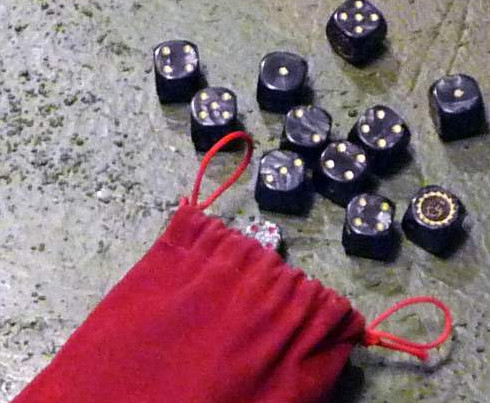
\includegraphics[width=\textwidth]{img/dice2-cropped.jpg}

        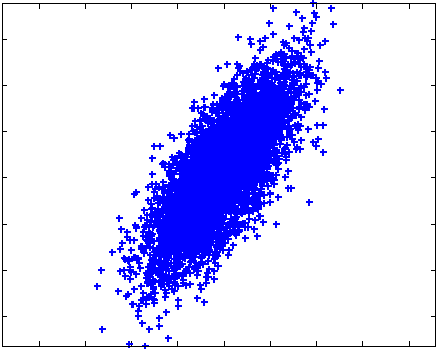
\includegraphics[width=\textwidth]{img/normal.png}
      \end{center}
    \end{column}
  \end{columns}
\end{frame}
